\section{Injections, Surjections, and Bijections} \label{S:typesoffunctions}
%\markboth{Chapter~\ref{C:functions}. Functions}{\ref{S:typesoffunctions}. Types of Functions}
\setcounter{previewactivity}{0}
%
Functions are frequently used in mathematics to define and describe certain relationships between sets and other mathematical objects.  In addition, functions can be used to impose certain mathematical structures on sets.  In this section, we will study special types of functions that are used to describe these relationships that are called injections and surjections.  Before defining these types of functions, we will revisit what the definition of a function tells us and explore certain functions with finite domains.

\begin{previewactivity}[\textbf{Functions with Finite Domains}] \label{PA:functionswithfinitedom} \hfill \\
Let  $A$  and  $B$  be sets.  Given a function  $f\x A \to B$, we know the following:

\begin{itemize}
\item For every  $x \in A$, $f( x ) \in B$.  That is, every element of  $A$  is an input for the function  $f$.  This could also be stated as follows:  For each  $x \in A$, there exists a  $y \in B$ such that  $y = f( x )$.

\item For a given $x  \in A$, there is exactly one  $y \in B$ such that  $y = f( x )$.

\end{itemize}
%\pagebreak
The definition of a function does not require that different inputs produce different outputs.  That is, it is possible to have  $x_1 , x_2  \in A$ with  
$x_1  \ne x_2 $ and  $f( {x_1 } ) = f( {x_2 } )$.  The arrow diagram for the function $f$ in Figure~\ref{fig:arrow63-1new} illustrates such a function.

\begin{figure}[h]
\begin{center}
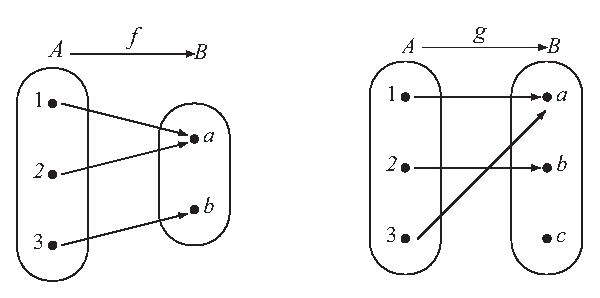
\includegraphics{figps-arrow63-1new.eps} 
\caption{Arrow Diagram for Two Functions} \label{fig:arrow63-1new}
\end{center}
\end{figure}

Also, the definition of a function does not require that the range of the function must equal the codomain.  The range is always a subset of the codomain, but these two sets are not required to be equal.  That is, if  
$g\x A \to B$, then it is possible to have a  $y \in B$ such that  $g( x ) \ne y$ for all  $x \in A$.  The arrow diagram for the function $g$ in Figure~\ref{fig:arrow63-1new} illustrates such a function.

Now let  $A = \left\{ {1,2,3} \right\}$, $B = \left\{ {a,b,c,d} \right\}$, and 
$C = \left\{ {s,t} \right\}$.  Define

\begin{center}
\begin{tabular}{c | c | c}
$f\x A \to B$ by &  $g\x A \to B$ by &  $h\x A \to C$ by \\
$f( 1 ) = a $  &  $g( 1 ) = a $  &  $h( 1 ) = s $ \\
$f( 2 ) = b $  &  $g( 2 ) = b $  &  $h( 2 ) = t $ \\
$f( 3 ) = c $  &  $g( 3 ) = a $  &  $h( 3 ) = s $
\end{tabular}
\end{center}
%
\begin{enumerate}
\item Which of these functions satisfy the following property for a function  $F$?

\begin{list}{}
\item For all  $x, y \in \text{dom}( F )$, if  $x \ne y$, then  
$F(x) \ne F(y)$.
\end{list}

\item Which of these functions satisfy the following property for a function  $F$?

\begin{list}{}
\item For all  $x, y \in \text{dom}( F )$, if  
$F( x ) = F( y )$, then  $x = y$.
\end{list}

\item Determine the range of each of these functions.

\item Which of these functions have their range equal to their codomain?

\item Which of the these functions satisfy the following property for a function  $F$?

\begin{list}{}
\item For all  $y$ in the codomain of $F$, there exists an  
$x \in \text{dom}( F )$ such that  $F( x ) = y$.
\end{list}
\end{enumerate}
\end{previewactivity}
\hbreak

\endinput

\begin{previewactivity}[\textbf{Statements Involving Functions}]
\label{PA:functionstatements} \hfill \\
Let $A$ and $B$ be nonempty sets and let $f\x A \to B$.  
In \typeu Activity~\ref*{PA:functionswithfinitedom}, we determined whether or not certain functions satisfied some specified properties.  These properties were written in the form of statements, and we will now examine these statements in more detail.
\begin{enumerate}
\item Consider the following statement:
\begin{list}{}
\item For all $x, y \in A$, if $x \ne y$, then $f ( x ) \ne f ( y )$.
\end{list}

\begin{enumerate} \label{PA:functionstatements1}
\item Write the contrapositive of this conditional statement.

\item Write the negation of this conditional statement.
\end{enumerate}

\item Now consider the statement:
\label{PA:functionstatements2}%
\begin{list}{}
\item For all $y \in B$, there exists an $x \in A$ such that $f ( x ) = y$.
\end{list}
Write the negation of this statement.

\item Let $g:\R \to \R$ be defined by $g ( x ) = 5x + 3$, for all $x \in \R$.  Complete the following proofs of the following propositions about the function $g$.
\label{PA:functionstatements3}

\newpar
\textbf{Proposition 1}.  For all $a, b \in \R$, if $g ( a ) = g ( b )$, then $a = b$.

\noindent
\textbf{\emph{Proof}}.  We let $a, b \in \R$, and we assume that 
$g ( a ) = g ( b )$ and will prove that $a = b$.  Since $g(a) = g(b)$, we know that
\[
5a + 3 = 5b + 3.
\]
(Now prove that in this situation, $a = b$.)

\newpar
\textbf{Proposition 2}.  For all $b \in \R$, there exists an $a \in \R$ such that $g ( a ) = b$.

\noindent
\textbf{\emph{Proof}}.  We let $b \in \R$.  We will prove that there exists an $a \in \R$ such that 
$g ( a ) = b$ by constructing such an $a$ in $\R$.  In order for this to happen, we need $g(a) = 5a + 3 = b$.

\noindent
(Now solve the equation for $a$ and then show that for this real number $a$, 
$g ( a ) = b$.)
\end{enumerate}

\end{previewactivity}
\hbreak

\endinput

\subsection*{Injections}
In previous sections and in \typeu Activity~\ref*{PA:functionswithfinitedom}, we have seen examples of functions for which there exist different inputs that produce the same output.   Using more formal notation, this means that there are functions  $f:A \to B$ for which there exist  \mbox{$x_1 , x_2  \in A$}
 with  $x_1  \ne x_2 $  and  $f( {x_1 } ) = f( {x_2 } )$.    
%What does it mean to say that this does not happen?  This was explored in Beginning Activity~\ref{PA:functionstatements}, and using the input-output version of a function, it means that if the inputs are different then the outputs are different.  More formally, it means that  if  $x_1  \ne x_2 $, then  
%$f( {x_1 } ) \ne f( {x_2 } )$.  
The work in the \typel activities was intended to motivate the following definition.
%
\begin{defbox}{injection}{Let  $f:A \to B$  be a function from the set  $A$  to the set  $B$.  The function  $f$  is called an \textbf{injection}
\index{injection}%
 provided that
\begin{center}
for all  $x_1 , x_2  \in A$, if  $x_1  \ne x_2 $, then  
$f( {x_1 } ) \ne f( {x_2 } )$.
\end{center}
When  $f$  is an injection, we also say that  $f$  is a \textbf{one-to-one function},
\index{one-to-one function}%
\index{function!one-to-one}%
 or that  $f$  is an \textbf{injective function}.}
\index{function!injective}%

\end{defbox}
%
Notice that the condition that specifies that a function  $f$  is an injection is given in the form of a conditional statement.  As we shall see, in proofs, it is usually easier to use the contrapositive of this conditional statement.  Although we did not define the term then, we have already written the contrapositive for the conditional statement in the definition of an injection in Part~(\ref{PA:functionstatements1}) of \typeu Activity~\ref*{PA:functionstatements}.  In that activity, we also wrote the negation of the definition of an injection.  Following is a summary of this work giving the conditions for  $f$  being an injection or not being an injection.

\begin{center}
\fbox{\parbox{4.68in}{
\begin{center}
\textbf{Let } $\boldsymbol{f\x A \to B}$\!.
\end{center}
\textbf{``The function $\boldsymbol{f}$ is an injection'' means that}
\begin{itemize}
\item For all  $x_1 , x_2  \in A$, if  $x_1  \ne x_2 $, then  
$f( {x_1 } ) \ne f( {x_2 } )$; or

\item For all  $x_1 , x_2  \in A$, if  $f( {x_1 } ) = f( {x_2 } )$, then  $x_1  = x_2 $.
\end{itemize}

\noindent
\textbf{``The function $\boldsymbol{f}$ is not an injection'' means that}
\begin{itemize}
\item There exist  $x_1 , x_2  \in A$ such that  $x_1  \ne x_2 $  and  
$f( {x_1 } ) = f( {x_2 } )$.
\end{itemize}
}}
\end{center}
%
%We will see how to use these ideas in the activities and examples that follow the discussion of surjections.
\begin{prog}[\textbf{Working with the Definition of an Injection}] \label{pr:injections} \hfill \\
Now that we have defined what it means for a function to be an injection, we can see that in 
Part~(\ref{PA:functionstatements3}) of \typeu Activity~\ref*{PA:functionstatements}, we proved that the function $g\x \R \to \R$ is an injection, where $g ( x ) = 5x + 3$ for all $x \in \R$.  Use the definition (or its negation) to determine whether or not the following functions are injections.
\begin{enumerate}
\item $k:A \to B$, where $A = \left\{a, b, c \right\}$, $B = \left\{1, 2, 3, 4 \right\}$, and 
$k (a) = 4$, $k(b) = 1$, and $k(c) = 3$.

\item $f:A \to C$, where $A = \left\{a, b, c \right\}$, $C = \left\{1, 2, 3\right\}$, and 
$f(a) = 2$, $f(b) = 3$, and $f(c) = 2$.

\item $F: \Z \to \Z$ defined by $F ( m ) = 3m + 2$ for all $m \in \Z$

\item $h: \R \to \R$ defined by $h ( x ) = x^2 - 3x$ for all $x \in \R$

\item $R_5 = \{0, 1, 2, 3, 4 \}$ and $s:R_5 \to R_5$ defined by $s ( x ) = x^3 \pmod 5$ for all $x \in R_5$.

\end{enumerate}
\end{prog}
\hbreak

\endinput

\subsection*{Surjections}
In previous sections and in \typeu Activity~\ref*{PA:functionswithfinitedom}, we have seen that there exist functions  $f\x A \to B$ for which $\text{range}(f) = B$.  This means that every element of $B$ is an output of the function $f$ for some input from the set $A$.  Using quantifiers, this means that for every $y \in B$, there exists an $x \in A$ such that $f( x ) = y$ . One of the objectives of the \typel activities was to motivate the following definition.  

%What does it mean to say that this does not happen?  One way to express this is to say that every element in the codomain is an output or that the codomain is equal to the range.  Using quantifiers, this means that  for every  
%$y \in B$, there exists an  $x \in A$  such that  $f( x ) = y$.
%
\begin{defbox}{surjection}{Let  $f\x A \to B$  be a function from the set  $A$  to the set  $B$.  The function  $f$  is called a \textbf{surjection}
\index{surjection}%
  provided that the range of  $f$   equals the codomain of  $f$.  This means that
\begin{center}
for every  $y \in B$, there exists an  $x \in A$  such that  $f( x ) = y$.
\end{center}
When  $f$  is a surjection, we also say that  $f$  is an \textbf{onto function}
\index{onto function}%
\index{function!onto}%
 or that  $f$  maps  $\boldsymbol{A}$  \textbf{onto}  $\boldsymbol{B}$\!.  We also say that  $f$  is a \textbf{surjective function}.}
\index{function!surjective}%
\end{defbox}
%
One of the conditions that specifies that a function  $f$  is a surjection is given in the form of a universally quantified statement, which is the primary statement used in proving a function is (or is not) a surjection.  Although we did not define the term then, we have already written the negation for the statement defining a surjection in Part~(\ref{PA:functionstatements2}) of \typeu Activity~\ref*{PA:functionstatements}.  We now summarize the conditions for  $f$  being a surjection or not being a surjection.
%
\begin{center}
\fbox{\parbox{4.68in}{
\begin{center}
\textbf{Let } $\boldsymbol{f\x A \to B}$\!.
\end{center}
\textbf{``The function $\boldsymbol{f}$ is a surjection'' means that}
\begin{itemize}
\item $\text{range}( f ) = \text{codom}( f ) = B$; or

\item For every  $y \in B$, there exists an  $x \in A$  such that  $f( x ) = y$.
\end{itemize}

\noindent
\textbf{``The function $\boldsymbol{f}$ is not a surjection'' means that}
\begin{itemize}
\item $\text{range}( f ) \ne \text{codom}( f )$; or

\item There exists a  $y \in B$ such that for all  $x \in A$, $f( x ) \ne y$.
\end{itemize}
}}
\end{center}
%
One other important type of function is when a function is both an injection and surjection.  This type of function is called a bijection.
\begin{defbox}{bijection}{A \textbf{bijection}
\index{bijection}%
 is a function that is both an injection and a surjection.  If the function  $f$  is a bijection, we also say that  $f$  is \textbf{one-to-one  and onto} and that  $f$  is a \textbf{bijective function}.}
\index{function!bijective}%
\end{defbox}

\begin{prog}[\textbf{Working with the Definition of a Surjection}] 
\label{pr:functionswithfinitedom} \hfill \\
Now that we have defined what it means for a function to be a surjection, we can see that in Part~(\ref{PA:functionstatements3}) of \typeu Activity~\ref*{PA:functionstatements}, we proved that the function $g: \R \to \R$ is a surjection, where $g ( x ) = 5x + 3$ for all $x \in \R$.  Determine whether or not the following functions are surjections.

\begin{enumerate}
\item $k\x A \to B$, where $A = \left\{a, b, c \right\}$, $B = \left\{1, 2, 3, 4 \right\}$, and 
$k (a) = 4$, $k(b) = 1$, and $k(c) = 3$.

\item $f\x \R \to \R$ defined by $f ( x ) = 3x + 2$ for all $x \in \R$.

\item $F\x \Z \to \Z$ defined by $F ( m ) = 3m + 2$ for all $m \in \Z$.

\item $s:R_5 \to R_5$ defined by $s ( x ) = x^3 \pmod 5$ for all $x \in R_5$.

\end{enumerate}
%\end{enumerate}
\end{prog}
\hbreak

\endinput

\subsection*{The Importance of the Domain and Codomain}
The functions in the next two examples will illustrate why the domain and the codomain of a function are just as important as the rule defining the outputs of a function when we need to determine if the function is a surjection.

\begin{example}[\textbf{A Function that Is Neither an Injection nor a Surjection}]\label{E:domainandcodomain} \hfill \\
Let  $f\x \mathbb{R} \to \mathbb{R}$  be defined by  $f( x ) = x^2  + 1$.  Notice that  
\[
f( 2 ) = 5  \text{ and } f( { - 2} ) = 5.
\]
This is enough to prove that the function  $f$  is not an injection since this shows that there exist two different inputs that produce the same output.

Since  $f( x ) = x^2  + 1$, we know that  $f( x ) \geq 1$ for all $x \in \mathbb{R}$.  This implies that the function  $f$  is not a surjection.  For example,  $ - 2$
  is in the codomain of  $f$  and  $f( x ) \ne  - 2$ for all  $x$  in the domain of  $f$\!.  
\end{example}

\begin{example}[\textbf{A Function that Is Not an Injection but Is a Surjection}]\label{E:domainandcodomain2} \hfill \\
Let  $T = \left\{ y \in \mathbb{R} \mid y \geq 1 \right\}$, and define  $F\x \mathbb{R} \to T$  by 
 $F( x ) = x^2  + 1$.
As in Example~\ref{E:domainandcodomain}, the function  $F$  is not an injection since  
$F( 2 ) = F( { - 2} ) = 5$.

Is the function  $F$ a surjection?  That is, does  $F$  map $\mathbb{R}$ onto  $T$?   As in Example~\ref{E:domainandcodomain}, we do know that  $F( x ) \geq 1$ for all 
$x \in \mathbb{R}$.  

To see if it is a surjection, we must determine if it is true that for every $y \in T$, there exists an $x \in \mathbb{R}$ such that $F ( x ) = y$.  So we choose  $y \in T$\!.  The goal is to determine if  there exists an $x \in \mathbb{R}$ such that
\[
\begin{aligned}
  F( x ) &= y \text{, or} \\ 
           x^2  + 1 &= y. \\ 
\end{aligned} 
\]
One way to proceed is to work backward and  solve the last equation (if possible) for  $x$.  Doing so, we get
\[
\begin{aligned}
  x^2  &= y - 1 \\ 
  x = \sqrt {y - 1} &\text{   or   }x =  - \sqrt {y - 1}.  \\ 
\end{aligned} 
\]
Now,  since  $y \in T$, we know that  $y \geq 1$  and hence that  $y - 1 \geq 0$.  This means that  $\sqrt {y - 1}  \in \mathbb{R}$.  Hence, if we use  $x = \sqrt {y - 1} $, then  $x \in \mathbb{R}$, and
\[
\begin{aligned}
  F( x ) &= F\left( {\sqrt {y - 1} } \:\right) \\ 
                    &= \left( {\sqrt {y - 1} } \: \right)^2  + 1 \\ 
                    &= ( {y - 1} ) + 1 \\ 
                    &= y. \\ 
\end{aligned}
\]
This proves that  $F$  is a surjection since we have shown that for all  $y \in T$\!, there exists an  $x \in \mathbb{R}$  such that  $F( x ) = y$.  Notice that for each $y \in T$\!, this was a constructive proof of the existence of an $x \in \mathbb{R}$ such that $F ( x ) = y$.
\end{example}
%\hbreak

\begin{center}
\fbox{\parbox{4.68in}{ 
%\begin{center}
\textbf{An Important Lesson}.  In Examples~\ref{E:domainandcodomain} and~\ref{E:domainandcodomain2}, the same mathematical formula was used to determine the outputs for the functions.  However, one function was not a surjection and the other one was a surjection.  This illustrates the important fact that whether a function is surjective depends not only on the formula that defines the output of the function but also on the domain and codomain of the function.
}}
\end{center}
The next example will show that whether or not a function is an injection also depends on the domain of the function.
%
\begin{example}[\textbf{A Function that Is an Injection but Is Not a Surjection}]\label{E:domainandcodomain3}  \hfill \\
Let  
$\mathbb{Z}^*  = \left\{ { {x \in \mathbb{Z}} \mid x \geq 0} \right\} = \mathbb{N} \cup \left\{ 0 \right\}$.  Define  $g\x \mathbb{Z}^*  \to \mathbb{N}$ by  
$g( x ) = x^2  + 1$.  (Notice that this is the same formula used in Examples~\ref{E:domainandcodomain} and~\ref{E:domainandcodomain2}.)  Following is a table of values for some inputs for the function  $g$.

\begin{center}
\begin{tabular}{ c | c  c  c | c}
  $x$ &  $g ( x )$ &   &  $x$ &  $g ( x )$ \\ \cline{1-2} \cline{4-5}
   0 &            1           &   &   3  &       10               \\ \cline{1-2} \cline{4-5}
   1 &            2           &   &   4  &       17               \\ \cline{1-2} \cline{4-5}
   2 &            5           &   &   5  &       26               \\ \cline{1-2} \cline{4-5}
\end{tabular}
\end{center}
Notice that the codomain is  $\mathbb{N}$, and the table of values suggests that some natural numbers are not outputs of this function.  So it appears that the function  $g$  is not a surjection.

To prove that   $g$  is not a surjection, pick an element of  $\N$  that does not appear to be in the range.  We will use  3, and we will use a proof by contradiction to prove that there is no $x$ in the domain $\left( \Z^*\right)$ such that  
$g( x ) = 3$.  So we assume that there exists an $x \in \Z^* $ with  $g( x ) = 3$.  Then
\begin{align*}
  x^2  + 1 &= 3 \\ 
       x^2 &= 2 \\ 
         x &=  \pm \sqrt 2.  \\ 
\end{align*}
But this is not possible since  $\sqrt 2  \notin \mathbb{Z}^* $.  Therefore, there is no 
$x \in \mathbb{Z}^* $ with  $g( x ) = 3$.  This means that for every  
$x \in \mathbb{Z}^* $,  $g( x ) \ne 3$.  Therefore,  3  is not in the range of  $g$,  and hence  $g$ is not a surjection.

The table of values suggests that different inputs produce different outputs, and hence that  $g$  is an injection.  To prove that  $g$  is an injection,  assume that  
$s, t \in \Z^* $ (the domain) with  $g( s ) = g( t )$.  Then
\begin{align*}
  s^2  + 1 &= t^2  + 1 \\ 
      s^2  &= t^2.  \\ 
\end{align*}
Since  $s, t \in \mathbb{Z}^* $, we know that  $s \geq 0\text{ and }t \geq 0$.  So the preceding equation implies that  $s = t$.  Hence,  $g$  is an injection.
\end{example}
%
\begin{center}
\fbox{\parbox{4.68in}{ 
%\begin{center}
\textbf{An Important Lesson}.  The functions in the three preceding examples all used the same formula to determine the outputs.  The functions in Examples~\ref{E:domainandcodomain} and~\ref{E:domainandcodomain2} are not injections but the function in Example~\ref{E:domainandcodomain3} is an injection.  This illustrates the important fact that whether a function is injective not only depends on the formula that defines the output of the function but also on the domain of the function.
}}
\end{center}


\begin{prog}[\textbf{The Importance of the Domain and Codomain}] 
\label{pr:domainandcodomain} \hfill \\
Let $\R^+ = \{ y \in \R \mid y > 0 \}$.  Define  
\begin{list}{}
\item $f \x \R \to \R$ by $f(x) = e^{-x}$, for each $x \in \R$, and
\item $g \x \R \to \R^+$ by $g(x) = e^{-x}$, for each $x \in \R$.
\end{list}
\end{prog}
Determine if each of these functions is an injection or a surjection.  Justify your conclusions.  \note Before writing proofs, it might be helpful to draw the graph of $y = e^{-x}$.  A reasonable graph can be obtained using $-3 \leq x \leq 3$ and $-2 \leq y \leq 10$.  Please keep in mind that the graph does not prove any conclusion, but may help us  arrive at the correct conclusions, which will still need proof.
%\subsection*{Another Important Lesson}
%The functions in the three preceding examples all used the same formula to determine the outputs.  The functions in Examples~\ref{E:domainandcodomain} and~\ref{E:domainandcodomain2} are not injections but the function in Example~\ref{E:domainandcodomain3} is an injection.  This illustrates the important fact that whether a function is injective not only depends on the formula that defines the output of the function but also on the domain of the function.
\hbreak
%

\endinput

\section*{Working with a Function of Two Variables}
It takes time and practice to become efficient at working with the formal definitions of injection and surjection.  As we have seen, all parts of a function are important (the domain, the codomain, and the rule for determining outputs).  This is especially true for functions of two variables.


For example, we define  $f\x \mathbb{R} \times \mathbb{R} \to \mathbb{R} \times \mathbb{R}$  by  
\[
f( {a, b} ) = ( {2a + b, a - b} )  \text{ for all } 
( {a, b} ) \in \R \times \R.
\]

Notice that both the domain and the codomain of this function are the set  
$\mathbb{R} \times \mathbb{R}$.  Thus, the inputs and the outputs of this function are ordered pairs of real numbers.  For example,
\[
 f( {1, 1} ) = ( {3, 0} ) \quad \text{and} \quad f( { - 1, 2} ) = ( {0,  - 3} ). \\ 
\]
To explore whether or not  $f$  is an injection, we assume that  
$( {a, b} ) \in \mathbb{R} \times \mathbb{R}$, 
$( {c, d} ) \in \mathbb{R} \times \mathbb{R}$, and   
$f( {a, b} ) = f( {c, d} )$.  This means that
\[
( {2a + b, a - b} ) = ( {2c + d, c - d} ).
\]
Since this equation is an equality of ordered pairs, we see that
\[
\begin{aligned}
   2a + b &= 2c + d\text{\!, and} \\ 
    a - b &= c - d\!. \\ 
\end{aligned}
\]
By adding the corresponding sides of the two equations in this system, we obtain  $3a = 3c$ and hence, $a = c$.  Substituting  $a = c$ into either equation in the system give us  $b = d$.  Since  $a = c$
  and   $b = d$, we conclude that
\[
( {a, b} ) = ( {c, d} ).
\]
Hence, we have shown that if $f( {a, b} ) = f( {c, d} )$, then  
$( {a, b} ) = ( {c, d} )$.  Therefore,  $f$  is an injection.

Now, to determine if  $f$  is a surjection, we let  
$( {r, s} ) \in \mathbb{R} \times \mathbb{R}$, where  $( {r, s} )$ is considered to be an arbitrary element of the codomain of the function  $f$.  Can we find an ordered pair $( {a, b} ) \in \mathbb{R} \times \mathbb{R}$ such that  $f( {a, b} ) = ( {r, s} )$?  Working backward, we see that in order to do this, we need
\[
( {2a + b, a - b} ) = ( {r, s} ).
\]
That is, we need
\[
  2a + b = r \quad \text{and} \quad    a - b = s. 
\]
Solving this system for  $a$  and  $b$  yields  
\[
a = \frac{{r + s}}{3} \text{ and } b = \frac{{r - 2s}}{3}.
\]
Since  $r, s \in \mathbb{R}$, we can conclude that  $a \in \mathbb{R}$ and 
$b \in \mathbb{R}$ and hence that  
\mbox{$( {a, b} ) \in \mathbb{R} \times \mathbb{R}$}.  We now need to verify that for these values of  $a$  and  $b$, we get  
$f( {a, b} ) = ( {r, s} )$.  So
\[
\begin{aligned}
  f( {a, b} ) &= f\!\left( {\frac{{r + s}}{3}, \frac{{r - 2s}}{3}} \right) \\ 
                         &= \left( {2\left( {\frac{{r + s}}{3}} \right) + \frac{{r - 2s}}{3},                             \frac{{r + s}}{3} - \frac{{r - 2s}}{3}} \right) \\ 
                         &= \left( {\frac{{2r + 2s + r - 2s}}{3}, \frac{{r + s - r + 2s}}{3}}                             \right) \\ 
                         &= ( {r, s} ). \\ 
\end{aligned} 
\]
This proves that for all  $( {r, s} ) \in \mathbb{R} \times \mathbb{R}$, there exists  $( {a, b} ) \in \mathbb{R} \times \mathbb{R}$ such that  
$f( {a, b} ) = ( {r, s} )$.  Hence, the function  $f$  is a surjection.  Since  $f$  is both an injection and a surjection,  it is a bijection.
\hbreak

\begin{prog}[\textbf{A Function of Two Variables}] 
\label{pr:function2variables} \hfill \\
Let $g \x \R \times \R \to \R$ be defined by $g(x, y) = 2x + y$, for all $(x, y) \in \R \times \R$.  

\noindent
\note Be careful! One major difference between this function and the previous example is that for the function $g$, the codomain is $\R$, not $\R \times \R$.  It is a good idea to begin by computing several outputs for several inputs (and remember that the inputs are ordered pairs).

\begin{enumerate}
  \item Notice that the ordered pair $(1, 0) \in \R \times \R$.  That is, $(1, 0)$ is in the domain of $g$.  Also notice that $g(1, 0) = 2$.  Is it possible to find another ordered pair $(a, b) \in \R \times \R$ such that $g(a, b) = 2$?  %What does this imply about the function $g$?

  \item Let $z \in \R$.  Then $(0, z) \in \R \times \R$ and so $(0, z) \in \text{dom } (g)$.  Now determine $g(0, z)$.

  \item Is the function $g$ an injection?  Is the function $g$ a surjection?  Justify your conclusions.
\end{enumerate}
 
\end{prog}
\hbreak
\endinput




%\begin{activity}[Injections, Surjections, and Bijections] \label{A:injsurjbi} \hfill \\
%For each of the following functions, construct a table of values using at least five different elements of the domain.  Then determine if the function is an injection, surjection, or bijection.
%
%
%\begin{multicols}{2}
%\begin{enumerate}
%\item $f\x \mathbb{R} \to \mathbb{R}$ by  $f( x ) = e^{ - x}$
%
%\item $f\x \mathbb{R} \to ( {0, + \infty } )$ by  \\$f( x ) = e^{ - x}$
%
%\item $f\x \mathbb{R} \to \mathbb{R}$  by  $f( x ) = e^{ - x^2 } $
%
%\item $f\x \mathbb{R} \to \left[ {0, + \infty } \right)$ by  \\$f( x ) = x^2$
%
%\item $f\x \left[ {0, + \infty } \right) \to \left[ {0, + \infty } \right)$  by \\ 
%$f( x ) = x^2 $
%
%\item $g\x \mathbb{R} \to \mathbb{R}$  by  $g( x ) = \sqrt[3]{{2x - 3}}$
%
%\item $s\x \mathbb{Z} \to \mathbb{Z}$  by  $s( x ) = 2x + 1$
%
%\item $f\! \x \! \left[ {\dfrac{{ - \pi }}{2}, \dfrac{\pi }{2}} \right] \to \left[ { - 1,\;1} \right]$
% by  $f( x ) = \sin x$
%
%%\item $g:\mathbb{Z} \to \left\{ {0, 1} \right\}$ by  \\
%%$g( x ) = \left\{ \begin{gathered}
%%  0\text{ if }x\text{ is even} \hfill \\
%%  1\text{ if }x\text{ is odd} \hfill \\ 
%%\end{gathered}  \right.$
%\end{enumerate}
%\end{multicols}
%%
%For example, the first function is an injection but is not a surjection.  Since this is a real function, a graph can be used to suggest these facts.  To prove that it is an injection, we assume that   $s, t \in \mathbb{R}$ with  $f( s ) = f( t )$.  Then
%\[
%e^{ - s}  = e^{ - t}.
%\]
%Taking the natural logarithm of both sides of the equation yields
%\[
%\begin{aligned}
%  \ln \!\left( {e^{ - s} } \right) &= \ln \!\left( {e^{ - t} } \right) \\ 
%                                - s&=  - t \\ 
%                                 s &= t. \\ 
%\end{aligned}
%\]
%This proves that  $f$  is an injection.  Also, since  $e^{ - x}  > 0$ for all  
%$x \in \mathbb{R}$, we can conclude that  $f( x ) > 0$ for all  
%$x \in \mathbb{R}$.  This means that the range of  $f$  is not equal to  $\mathbb{R}$
%and hence  $f$  is not surjective.
%\end{activity}
%\hbreak
%









\endinput


\begin{center}
\setlength{\unitlength}{0.3cm}
\begin{picture}(14,14)
\put(2,6){\oval(4,12)}
\put(10,6){\oval(4,8)}

\put(2,2){\circle*{.5}}
\put(2,6){\circle*{.5}}
\put(2,10){\circle*{.5}}

\put(10,4){\circle*{.5}}
\put(10,8){\circle*{.5}}

\put(1,1.8){3}
\put(1,5.8){2}
\put(1,9.8){1}
\put(10.5,3.8){$b$}
\put(10.5,7.8){$a$}

\put(1.8,12.5){$A$}
\put(10,12.5){$B$}

\put(3,12.8){\vector(1,0){7}}
\put(6,13.2){$f$}

\put(2.5,2){\vector(4,1){7.1}}
\put(2.5,6){\vector(4,1){7.1}}
\put(2.5,10){\vector(4,-1){7.1}}

\end{picture}
\end{center}

\begin{center}
\setlength{\unitlength}{0.3cm}
\begin{picture}(14,14)
\put(2,6){\oval(4,12)}
\put(10,6){\oval(4,12)}

\put(2,2){\circle*{.5}}
\put(2,6){\circle*{.5}}
\put(2,10){\circle*{.5}}

\put(10,2){\circle*{.5}}
\put(10,6){\circle*{.5}}
\put(10,10){\circle*{.5}}

\put(1,1.8){3}
\put(1,5.8){2}
\put(1,9.8){1}
\put(10.5,1.8){$c$}
\put(10.5,5.8){$b$}
\put(10.5,9.8){$a$}

\put(1.8,12.5){$A$}
\put(10,12.5){$B$}

\put(3,12.8){\vector(1,0){7}}
\put(6,13.2){$g$}

\put(2.7,2){\vector(1,1){7.2}}
\put(2.5,6){\vector(1,0){7.1}}
\put(2.5,10){\vector(1,0){7.1}}

\end{picture}
\end{center}


\[
\BeginTable
\BeginFormat
| p(2.5in) | p(2.5in) |
\EndFormat
" {\bf 1}. $f:\mathbb{R} \to \mathbb{R}$ by  $f( x ) = e^{ - x}$. " 
{\bf 6}. $g:\mathbb{R} \to \mathbb{R}$  by  $g( x ) = \sqrt[3]{{2x - 3}}$. " \\+04
" {\bf 2}. $f:\mathbb{R} \to ( {0, + \infty } )$ by  \\$f( x ) = e^{ - x}$. " {\bf 7}. $s:\mathbb{Z} \to \mathbb{Z}$  by  $s( x ) = 2x + 1$. " \\+04
" {\bf 3}. $f:\mathbb{R} \to \mathbb{R}$  by  $f( x ) = e^{ - x^2 } $. " 
{\bf 8}. $f:\left[ {\dfrac{{ - \pi }}{2}, \dfrac{\pi }{2}} \right] \to \left[ { - 1,\;1} \right]$
 by  $f( x ) = \sin x$. " \\+04
\EndTable
\]




